\section{Modernizacja sposobu pobierania obrazu z kamery} 
\label{sec:img-acq}
W celu zwiększenia możliwości robota Dark Explorer w dziedzinie przetwarzania
obrazu niezbędne było polepszenie rozdzielczości zdjęć otrzymywanych z wbudowanej
kamery. W wersji bazowej maksymalne rozdzielczości z jakimi było możliwe
pobieranie obrazów to 160x100 pikseli w kolorze oraz 320x200 pikseli w odcieniach
szarości. Wartości te~zostały najprawdopodobniej narzucone przez ograniczenia
pamięci podręcznej mikrokontrolera ARM, który posiada jedynie 64kB szybkiej
pamięci SRAM. Ilość ta wystarczyła na pobranie maksymalnie $320*200=64000$ bajtów
danych pozostawiając 1536 bajtów na zmienne niezbędne do poprawnego działania
oprogramowania systemu wbudowanego.

Wykorzystywana kamera posiada osiem wyjść równoległych odpowiadających za~jeden
bajt danych. Wszystkie osiem bitów na wyjściu zmienia się z każdym taktem zegara
sterującego kamery, podanego na jej wejście. W taki sposób z każdym cyklem 
zegara, kamera oddaje do naszej dyspozycji dane z kolejnej porcji obrazu. W
konfiguracji początkowej zegar wejściowy kamery był tworzony w sposób czysto
programowy. Jedno z wyjść GPIO mikrokontrolera było ustawiane na przemian raz w
stan wysoki, a raz w stan niski. Niewątpliwie podejście to znacząco ułatwia
synchronizację pomiędzy sygnałem zegarowym a momentem pobierania danych
eliminując możliwość wczytania danych z wyjścia kamery w momencie w którym
wyjścia te są w stanie nieustalonym.

\begin{figure}[ht!]
 \centering 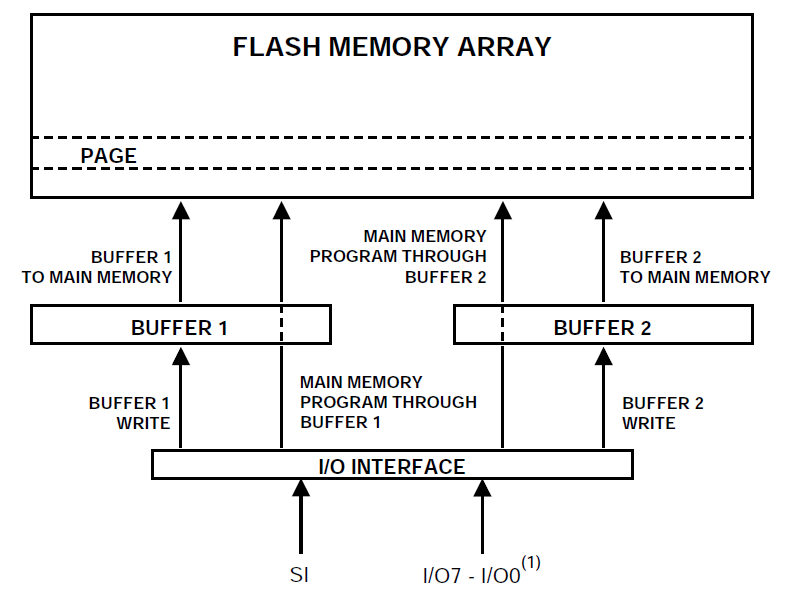
\includegraphics[height=85mm]{../images/ch04/dataflash_structure.png}
 \caption{Schemat struktury logicznej AT45DB321B wraz z zaznaczonymi operacjami zapisu\cite{AT45DB321BApplicationNote}.}
 \label{fig:DataFlashStruct}
\end{figure}

Przedstawiony problem niedostatecznej ilości pamięci został rozwiązany poprzez
wykorzystanie pamięci Data Flash wbudowanej w moduł mikrokontrolera. Użyty układ
AT45DB321B\cite{AT45DB321BDataSheet} dostarcza 32 megabitów pamięci którą możemy
zarządzać poprzez interfejs szeregowy SPI\footnote{SPI -- Serial Peripheral
Interface Bus}. Zastosowana pamięć posiada dwa bufory po 528 bajtów pojemności.
Struktura logiczna AT45DB321B wraz z zaznaczonymi operacjami zapisu została
przedstawiona na rysunku \ref{fig:DataFlashStruct}.  Podczas przenoszenia danych
z jednego bufora do pamięci Data Flash możliwy jest zapis informacji do drugiego
bufora. W ten sposób jest emulowany zapis danych do pamięci Data Flash w trybie
ciągłym. Zarys algorytmu ciągłego zapisu danych do AT45DB321B przedstawia schemat
na rysunku \ref{fig:DataFlashConstantWrite}

\begin{figure}[ht!]
 \centering
 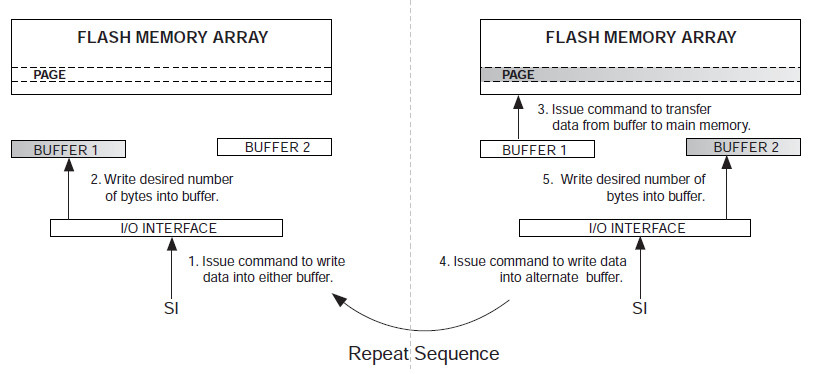
\includegraphics[height=70mm]{../images/ch04/dataflash_constant_write.png}
 \caption{Schemat procedury ciągłego zapisu do układu AT45DB321B\cite{AT45DB321BApplicationNote}.}
 \label{fig:DataFlashConstantWrite}
\end{figure}

Czas zapisu danych na stronie pamięci układu AT45DB321B nie jest stały. Wymusza
to zmianę podejścia do zegara sterującego kamerą z koncepcji programowej na~sprzętową, tak aby okres zegara był stały. Niejednorodny zegar spowodowałby
przebarwienia na obrazie wynikające ze sposobu działania mechanizmu dobierania
ekspozycji, wbudowanego w kamere PO6030K. W celu uzyskania sprzętowego zegara
zostało użyte urządzenie peryferyjne mikrokontrolera AT91SAM7S generujące
sygnał prostokątny o określonej częstotliwości. Z powodu multipleksowania tego
urządzenia z jednym z pinów GPIO mikrokontrolera podłączonego do wyjścia danych z
kamery, konieczne było zastosowanie przeplotu w taśmie podłączeniowej kamery w
celu dostarczenia odpowiednich sygnałów do prawidłowych wejść/wyjść.

Pojawiły się również problemy podczas uruchamiania interfejsu szeregowego SPI za
pomocą którego mikrokontroler komunikuje się z układem AT45DB321B. Okazało się
bowiem, że wyjścia/wejścia odpowiedzialne za obsługę tego interfejsu są
multipleksowane z wyjściami kontrolera PWM\footnote{PWM -- Pulse Width
Modulation} odpowiedzialnego za odpowiednie wysterowanie silników robota. W
konfiguracji podstawowej silniki te były kontrolowane przez 4 niezależne sygnały
PWM pozwalające na obracanie się każdego koła robota z inną prędkością.
Stwierdzono, iż taka funkcjonalność nie jest niezbędna i wykorzystano trzy zbędne
wyjścia sygnałów PWM do obsługi interfejsu SPI, a przy pomocy własnoręcznie
wykonanej zworki dostarczono jeden sygnał PWM dla wszystkich czterech silników.

Dane z kamery są początkowo umieszczane w pamięci SRAM do momentu uzbierania
grupy 512 bajtów (rozmiar strony pamięci układu AT45DB321B). Zabieg ten jest
wykonywany w celu poświęcenia jak najmniejszej ilości czasu na zapis do pamięci
Data Flash. Przygotowana grupa danych jest następnie przesyłana do AT45DB321B
poprzez interfejs SPI z wykorzystaniem mechanizmu DMA\footnote{DMA - Direct
Memory Access}.

Wszystkie podjęte kroki pozwoliły na odbiór obrazu o maksymalnych
rozdzielczościach oferowanych przez układ PO6030K to znaczy 640x480 pikseli w
odcieniach szarości oraz 640x480 pikseli w kolorze.